\documentclass[a4paper,12pt]{article}

\usepackage{amsmath}
\usepackage{graphicx}

\title{Scientific Calculator Experiment}
\date{\today}

\begin{document}
\author{M.Ranjith}
\maketitle

\section{Introduction}

This experiment aims to design a {scientific calculator} using a {16x2 LCD display}, {push buttons}, and a voltmeter} as input components. The calculator will be capable of performing basic arithmetic operations such as addition, subtraction, multiplication, and division, along with advanced mathematical functions like trigonometry and logarithms.

\subsection{Objective}
The primary objectives of this experiment are:
\begin{itemize}
    \item To interface a {16x2 LCD display} with a microcontroller.
    \item To use push buttons} for selecting mathematical operations.
    \item To utilize a {voltmeter} for inputting values.
    \item To program the microcontroller for performing scientific calculations.
\end{itemize}
\newpage 
\begin{frame}
\frametitle{Solution}
        \begin{figure}[h]
        \centering
       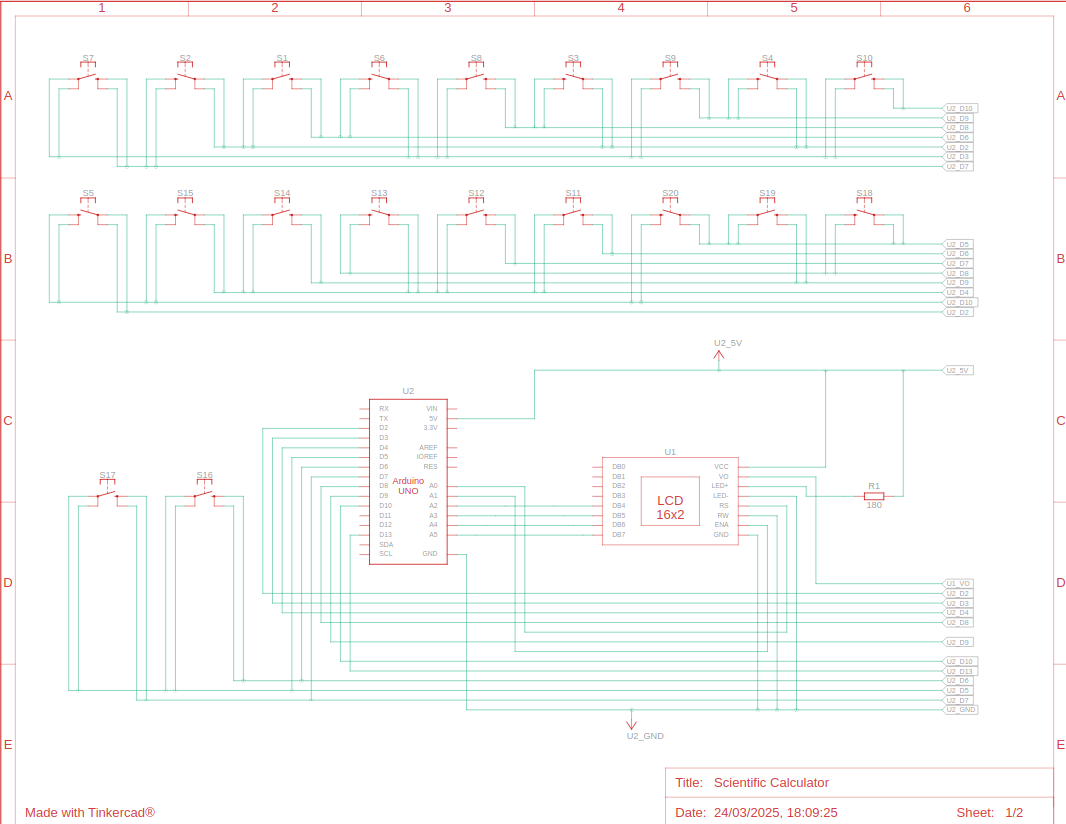
\includegraphics[width=0.5\linewidth]{figs/Circuit1.png}
       \caption{}
       \label{graph}
    \end{figure}
\end{frame}
\section{Required Materials}
The following components are required for the experiment:
\begin{itemize}
    \item {Microcontroller} (Arduino Uno/Nano)
    \item {16x2 LCD display} (for result display)
    \item {Push buttons} (for operation selection)
    \item {Voltmeter} (for numerical input)
    \item {Resistors} (1kΩ, 10kΩ)
    \item {Jumper wires}
    \item {Breadboard}
    \item {5V Power Supply} (from Arduino or external source)
\end{itemize}


\begin{table}[H]
    \centering
    \renewcommand{\arraystretch}{1.2} % Adjust row height
    \begin{tabular}{|c|c|}
        \hline
        \textbf{Component} & \textbf{Arduino Pin} \\
        \hline
        \multicolumn{2}{|c|}{\textbf{Button Matrix}} \\
        \hline
        Row 1 & 2 \\
        Row 2 & 3 \\
        Row 3 & 4 \\
        Row 4 & 5 \\
        Column 1 & 6 \\
        Column 2 & 7 \\
        Column 3 & 8 \\
        Column 4 & 9 \\
        Column 5 & 10 \\
        \hline
        \multicolumn{2}{|c|}{\textbf{Shift Button}} \\
        \hline
        Shift Button & 13 \\
        GND & GND \\
        \hline
        \multicolumn{2}{|c|}{\textbf{LCD Display (16x2, Non-I2C)}} \\
        \hline
        LCD RS & A0 \\
        LCD EN & A1 \\
        LCD D4 & A2 \\
        LCD D5 & A3 \\
        LCD D6 & A4 \\
        LCD D7 & A5 \\
        \hline
    \end{tabular}
    \caption{Circuit Connections of the Scientific Calculator}
    \label{tab:circuit_connections}
\end{table}
\newpage

\section{Procedure}

\subsection{Step 1: Circuit Connections}
\begin{enumerate}
    \item Connect the {16x2 LCD display} to the microcontroller:
    \begin{itemize}
        \item RS, E, D4-D7 pins → Arduino digital pins 7, 8, 9, 10, 11, 12.
        \item VSS to {GND}, VDD to {5V}.
    \end{itemize}
    \item Connect the {push buttons}:
    \begin{itemize}
        \item One button for each operation (+, -, ×, ÷).
        \item Connect one terminal to Arduino digital pins (2–5) and the other to GND using pull-down resistors (10kΩ).
    \end{itemize}
    \item Connect the {voltmeter} to an analog input pin (e.g., A0) to read voltage values.
\end{enumerate}
\subsection{Step 2: Programming the Microcontroller}
\begin{enumerate}
    \item Write and upload an Arduino program to:
    \begin{itemize}
        \item Read voltage values as input numbers.
        \item Detect button presses to determine operations.
        \item Perform calculations and display results on the 16x2 LCD.
    \end{itemize}
    \item Ensure the program updates the display after each operation.
\end{enumerate}

\subsection{Step 3: Testing and Observations}
\begin{enumerate}
    \item Input numbers using the voltmeter and verify correct readings.
    \item Press the operation buttons and confirm calculations.
    \item Ensure accurate results are displayed on the LCD.
\end{enumerate}

\section{Conclusion}

In this experiment, a scientific calculator was successfully built using a {16x2 LCD display}, {push buttons}, and a {voltmeter}. The microcontroller effectively handled arithmetic and scientific calculations based on user inputs. This experiment provided insights into:
\begin{itemize}
    \item Interfacing {LCD displays} and {push buttons} with a microcontroller.
    \item Using a {voltmeter} as an input device.
    \item Implementing real-time {mathematical computations} in embedded systems.
\end{itemize}

Future improvements could include adding a {keypad} for direct numerical input and incorporating more advanced mathematical functions.\
\ \\ \\
\textbf{code reference-{koushik muthyala}}
\end{document}
